\documentclass[12pt]{article}
\usepackage{graphicx}
\usepackage[margin=2cm]{geometry}
\usepackage{titlesec}
\usepackage{titling}
\usepackage{lipsum}
\usepackage{fancyhdr}
\usepackage{rotating}
\usepackage{hyperref}
\usepackage{enumitem}
\usepackage{tikz}
% \usepackage{standalone}
\usepackage{pdfpages}

\graphicspath{{./resources/}}

\newcommand{\bb}[1]{\textbf{\textit{#1}}}
\newcommand{\tco}{Touriscov}

\hypersetup{
    colorlinks=true,
    linkcolor=blue,
    filecolor=magenta,      
    urlcolor=cyan,
    pdftitle={miniMBAProject},
    pdfpagemode=FullScreen,
    }

\lhead{TOURISCOV}
\chead{}
\rhead{
\includegraphics[scale=0.1]{/miniMBA.png}}
\lfoot{}
\cfoot{\thepage}
\rfoot{}

\renewcommand{\thefigure}{}

\renewcommand{\maketitle}{
\begin{center}
    \Huge\textbf{Team 122} \\ 
    \vspace{1em}
    \Large\bfseries participant 1 \\
    {[Retracted]} \\
    \Large\bfseries participant 2\\
    {[Retracted]} \\
    \Large\bfseries participant 3 \\
    {[Retracted]} \\
    \Large\bfseries participant 4\\
    {[Retracted]} \\
    \Large\bfseries participant 5\\
    {[Retracted]} \\

    \vspace{1em}
    \large May 11\textsuperscript{th}, 2023
\end{center}
}


\title{MBA Assignment}
\author{Amr Wahdan}
\date{Thursday, May 11th 2023}

\begin{document}
\pagenumbering{0}

\begin{center}
   \topskip8cm
    
\includegraphics[width=0.8\textwidth]{uniLogo.jpg}  
\end{center}
\vspace{1em}
\begin{center}
    \scalebox{2}{\Huge\textbf{TOURISCOV}}
\end{center}
\vspace{1em}
\maketitle
\pagenumbering{roman}
\newpage

\begin{center}
   \topskip8cm
    
\includegraphics[width=0.5\textwidth]{miniMBA.png}  
\end{center}
\vspace{1em}

\begin{center}
    \Large\bfseries TOURISCOV --- A tourism-centered company
    \vspace{0.5em}
    \hrule\vspace{0.2em}\hrule
\end{center}

\begin{itemize}
    \item Touriscov is a start-up company focused on connecting adventure-seeking unorthodox tourists who enjoy discovering local rarely visited gems with passionate guides who lived through that history and/or witnessed it first-hand.
    \item We aim to centralize and expand the touristic experience of our users by allowing them to visit and read about various sites which they might have missed out on completely in a normal guided tour. We also introduce our users to new historical, cultural, and religious sites by employing sophisticated algorithms that use the power of AI \& machine-learning to recommend new places to our users.
    \item Our plan is to disrupt the tourism market, and to get in on the untapped market of under-privileged tourists who cannot afford international travel. Touriscov allows those segment of tourists to reap the joys of local tourism which they might have missed out on otherwise.
    \item Touriscov relies mostly on local guides --- guides who might not have undergone a formal college education in history and/or education. While those guides might not have been enrolled in a history course before, they balance that by being very passionate and by the fact that most often than not they have lived through what they are talking about; saw it first-hand; or knew a close relative who knows all about the subject at hand. 
    \item The introduction of Touriscov, its services and subsidiaries to a given country will --- without a doubt --- enhance and expand the tourism market in said country. And it will also expand the list of tourist sites by shedding a light on lesser-known sites and/or touristy areas. 
\end{itemize}


\newpage
\pagenumbering{arabic}
\pagestyle{fancy}
\topskip2cm
\section{Why Touriscov}
\begin{enumerate}[label= \roman*.]
    \item \textbf{\textit{Niche Sites}}: Many interesting, culturally and historically relevant sites all around the globe are missing from the eyes of international and local tourists due to their niche significance and/or their lesser known status. For instance, many Sufi shrines that are pretty religiously significant to a large swath of people who are interested in Islam or just generally in religious tourism, go undiscovered and untalked about. Touriscov aims to bring sites like these to the public eye and capitalize on that new emerging market.
    \item \textbf{\textit{Untapped market}}: While tourism is a joyful and intellectually stimulating experience, it is --- unfortunately --- not always accessible to most people. Especially those under economic pressure. Touriscov aims to allow those users to experience some of the fun of tourism --- admittedly limited --- by introducing them to local sites they do not need to travel to. 
    \item \textbf{\textit{Cultural Exchange}}: Touriscov also aims to further the cultural exchange among its multi-cultural user-base by setting up annual and monthly events to connect like-minded people from all over the globe.
    \item \textbf{\textit{Democratization of Tourism}}: Knowledge is money. And here at Touriscov, we allow our local guides to share their passion for history and their lived experiences for a fee of their choosing. This allows our guides to talk about topics they are passionate about, while also making a living off their passion.
    \item \textbf{\textit{Free and accessible Documentation}}: Unfortunately for humanity, not all history is documented. Many local historical sites are left as-is for centuries without a ceramic plaque to describe them for the curious among us --- and not even a mention online sometimes. Touriscov aims to change that by empowering the forces that fueled the rise of Wikipedia. Our crowd-written database will cover many undeservedly unheard of sites. And we will ensure historical accuracy by employing historians and fact-checkers to check all its entries. 
    \item \textbf{\textit{Safety \& Well-being tips}}: Tourism is lovely, but only so when it is done in a safe way. And unfortunately for many people out there, that is not the case. Women \& minorities of all kinds are constantly faced with barriers that hinder their enjoyment of tourism. Touriscov provides forums that allows these groups to share their experience and demand change from the hosting country.
\end{enumerate}

\newpage

\section{Business Model Canvas}
A graphical representation of Touriscov business model is included in the appendix \par

\subsection{Customer Segments}
\tco\ plans to have a wide and varied customer base to meet the needs of everyone out there. To achieve that goal, \tco\  targets multiple segments of society with specific offers tailored to their wants and needs.\ \par 

\subsubsection{16+ Youth}
For instance, \tco\ targets the youth by giving them discounts for historical and culturally significant sites they are studying at school and/or college. This serves \tco\ bottom line, while also enriching the society \tco\ operates in.\ \par

\subsubsection{Low-income segments}
\tco\ also targets some low-income segments of society --- segments which are usually deprived of the joys of tourism due to the high cost of travel. These segments are targeted by introducing them to affordable travel-free sites, and by offering them coupons based on website traffic and on-site activities like using \tco\ services more, writing reviews \& taking pictures and uploading them to the website.\ \par 

\subsubsection{Adventure Seekers}
This minor yet vital segment of society is also targeted by offering compound bonuses --- bonuses that double or generally grow in value the more you travel and visit new places.\ \par
\noindent
This segment is very much on top of \tco\ list to win over since this segment alone is capable of fueling \tco\ ad campaign and bringing over new users.\ \par

\subsubsection{Niche Segments}
Other niche segments are targeted by offering them specific incentives to use Touriscov's services

\subsection{Customer Relationships}

\subsubsection{Self-service}
\tco\ interacts with its customers in a mostly self-service fashion through the company website. An average customer can benefit from \tco\ services mostly on their own without interacting with any \tco\ representative. This is both a win for the customer who knows his needs best and can best fill them by finding their way on the company website. And it is also best for \tco\ who saves on this unnecessary labor costs.

\subsubsection{Retail stores}
There are also a few select retail outlets \tco\ plans to operate. These stores are meant to facilitate customer service interactions like answering questions, solving problems, and helping technically-challenged customers find their way on the company website. 


\subsection{Value proposition}
\subsubsection{For the hosting country}
The main thing \tco\ plans to offer to the tourism industry and the hosting country as a whole is the reviving of old lesser-known sites, and the much-lacking documentation for both well-known and under-appreciated sites. These two things can transform the tourism industry in any given country by ramping up local and international tourism and ensuring a high-quality experience for both kinds of tourists.\ \par

\subsubsection{For the customer}
The average tourist is bound to benefit from the introduction of \tco\ to the country to which they plan to visit. For one, they will find enough information on \tco\ that will allow them to choose their destination in a way that aligns with their wants, needs, and capabilities. And secondly, \tco\ will take on the role of local governments when governments fail to provide adequate care to incoming tourists. This will inevitably help out developing nations that have overloaded \& under-equipped governments --- and sometimes corrupt governments --- revamp their tourism industry or usher in a new one. And clearly, this will provide customers access to history that they would not have had access to otherwise.

\subsection{Key Resources}
Touriscov's business model doesn't require a lot of inputs to produce value. The only two resources that are vital to \tco\ are an educated populous from which \tco\ can hire its employees and expand its human capital, and credit processors like \textit{Visa} \& \textit{MasterCard}.


\subsection{Key Activities}

 \begin{itemize}
     \item \bb{Travel Recommendations} Touriscov's algorithms that are based on sophisticated AI \& Machine learning will make use of customer activity on the company website to recommend them travel destinations, activities, and special offers.
     \item \bb{Documentation of sites} As previously mentioned, documenting sites --- especially lesser-known ones --- is one of Touriscov's key activities. Having a small QR code sticker substitute big ceramic plaques will be both efficient and cost-effective. 
     \item \bb{Online Forums} Reviews are essential for any customer, when it comes to planning vacations or tourism trips in general. So, \tco\ plans to host regulated online forums on which customers can share ideas and exchange tips.
     \item \bb{Cultural Events} Holding annual and monthly cultural events is also something \tco\ plans to do. These will function as a marketing gimmick and will help expand Touriscov's outreach and its customer base.
 \end{itemize}

\subsection{Key Partners}

\begin{itemize}
    \item \bb{Credit processors} \textit{Visa} \& \textit{MasterCard}, and other credit processors are essential for facilitating transactions made via the company website.
    \item \bb{Transportation companies} Partnering with a good bussing company and a reputable airline company will help smooth the conversion rate of website traffic to customers by making it easy to book your transit just after making your decision on the website. 
    \item \bb{Hotels} Same line of argument applies to hotels. Partnering with a good hotel company will make it possible for customers to book their entire trip from start to finish on Touriscov's website.
    \item \bb{Local Museums} Partnering with local museums is essential to Touriscov's success. Museums will make the backbone of Touriscov's documentation effort and will ensure the factual correctness of the information residing there on the website.
    \item \bb{Tech Companies} This goes without saying, but \tco\ will \textit{need} to partner with a good tech/IT company to build and maintain its extensive website.
    \item \bb{AWS} Amazon Web Services will be the main hosting provider for \tco.
\end{itemize}

\subsection{Revenue Streams}
\tco\ will have multiple abundant revenue streams 

\subsubsection{Middleman fees}
These are the generated revenue \tco\ will make by acting as the middleman between the customer and another company.\ \tco\ will take a small cut from each successful transaction made on the company website.
\begin{itemize}
    \item Flight bookings
    \item Bus ticketing
    \item Hotel reservations
    \item Museums' ticketing
    \item etc.
\end{itemize}

\subsubsection{Subscription fees}
\tco\ plans to sell a subscription service that will offer subscribers monthly packages to choose from. These packages will have fully-paid and fully-prepped vacations and adventures that customers can enjoy. These packages will help \tco\ make use of its purchasing power that makes use of the \href{https://www.wikiwand.com/en/Economies_of_scale}{Economies of Scale} effect and the cost savings related to that.

\subsubsection{Bid data sales}
\tco\ will operate a massive Big-data Center that will have all of its user data that it keeps track of. These data fuels Touriscov's recommendation algorithms. And it will also be valuable for many other companies and research centers.
\subsubsection{Ad revenue}
A lot of revenue will be generated by making use of Touriscov's virtual real-estate. The company website will have lots of valuable ad space that many companies --- and even government agencies/ministries --- will pay lots of money for.

\subsection{Cost Structure}
\tco\ is mainly a \textit{cost-driven} business as opposed to a \textit{value-driven} business which means that \tco\ focuses more on lowering the costs of its products as opposed to delivering the highest quality out there. In less words, \tco\ competes on the cost front rather than the value front.\ \tco\ costs split into various types, but the main two distinctions are \textit{Fixed costs} \& \textit{Variable costs}
\subsubsection{Fixed costs}
\begin{itemize}
    \item Web hosting costs
    \item Retail stores rent
    \item Employee salaries
\end{itemize}

\subsubsection{Variable costs}
\begin{itemize}
    \item Marketing costs
    \item Special events
    \item Website maintenance
\end{itemize}

\section{Company Structure \& legalities}
\tco\ plans to start as a partnership like most small businesses out there and then transform into an LLC\@. The decision to start as a partnership is taken so as to simplify our startup process, fill less government forms, and get to work as fast as possible. And the decision to transform into an LLC after a while is planned so \tco\ could access more funds by being publicly traded on the stock market, and to allow \tco\ to expand easily into foreign markets.

\section{Competition}

\noindent

\begin{minipage}{.5\textwidth}
The main competitor for Touriscov is the somewhat well-known \href{https://www.tripadvisor.com/}{Tripadvisor}, which has the lion's share of the market.\ \par

Tripadvisor has a similar business model to Touriscov in that it also operates online forums that enable tourists from around the globe to find new sites, and it too collaborates with the local guide community in each country to facilitate tours for incoming tourists.\ \par

Another lesser known competitor is \href{https://www.expedia.com/}{Expedia Travel}. Unlike Tripadvisor, however, Expedia does not have similar business model to Touriscov and both work more or less in parallel.\ \par

Aside from these main two competitors, there are some companies out there who could be classified as competition in a loose sense. For example, the famous hotel-booking company \href{https://www.booking.com/}{Booking.com} is one of those. And the lesser known \href{https://www.tripexpert.com/}{Tripexpert} is also somewhat of a competitor since it also offers travel reviews. But unlike the previously mentioned TripAdvisor, its reviews are editorialized i.e.\ it is written by professionals.

\end{minipage}%
\hfill
\begin{minipage}{.5\textwidth}
\begin{flushright}
  \begin{center}
  \vspace{1em}
    
\includegraphics[scale=0.2]{tripadvisor-logo.png}
    
\includegraphics[scale=0.9]{expedia_logo.jpg}
  \end{center}
  \end{flushright}
\end{minipage}


\subsection{What sets Touriscov apart}
\begin{itemize}
    \item \textbf{\textit{Niche unknown sites}} None of our competitors caters to tourists with niche interests and promotes unknown sites like \tco\ does.
    \item \textbf{\textit{Dox}} None of our competitors offers free accessible documentation --- especially of lesser-known sites --- that could be accessed easily through a sticker QR code
    \item \textbf{\textit{Incentives}} None of our competitors offers incentives to fuel demand and attract customers from untapped markets like \tco\ does.
\end{itemize}


\section{Nitty-Gritty Finances}
The following is a loose description of the finances of \tco\ is staring with an initial capital of 150k. And those 150k are divvied up into three buckets: investment capital, working capital, and events fund.\ \par

\noindent
And each one of those is divvied up further into sub buckets detailing the costs \tco\ will endure to be a successful startup.\ \par

\noindent
By far the biggest cost for \tco\ is the Documentation costs since \tco\ will have to collaborate with universities and museums to get that done with a high degree of accuracy.\ \par

\begin{center}
    \textbf{Note that the numbers for the working capital are calculated per month}
\end{center}

\vspace{1em}

\begin{figure}[h]
    \centering
    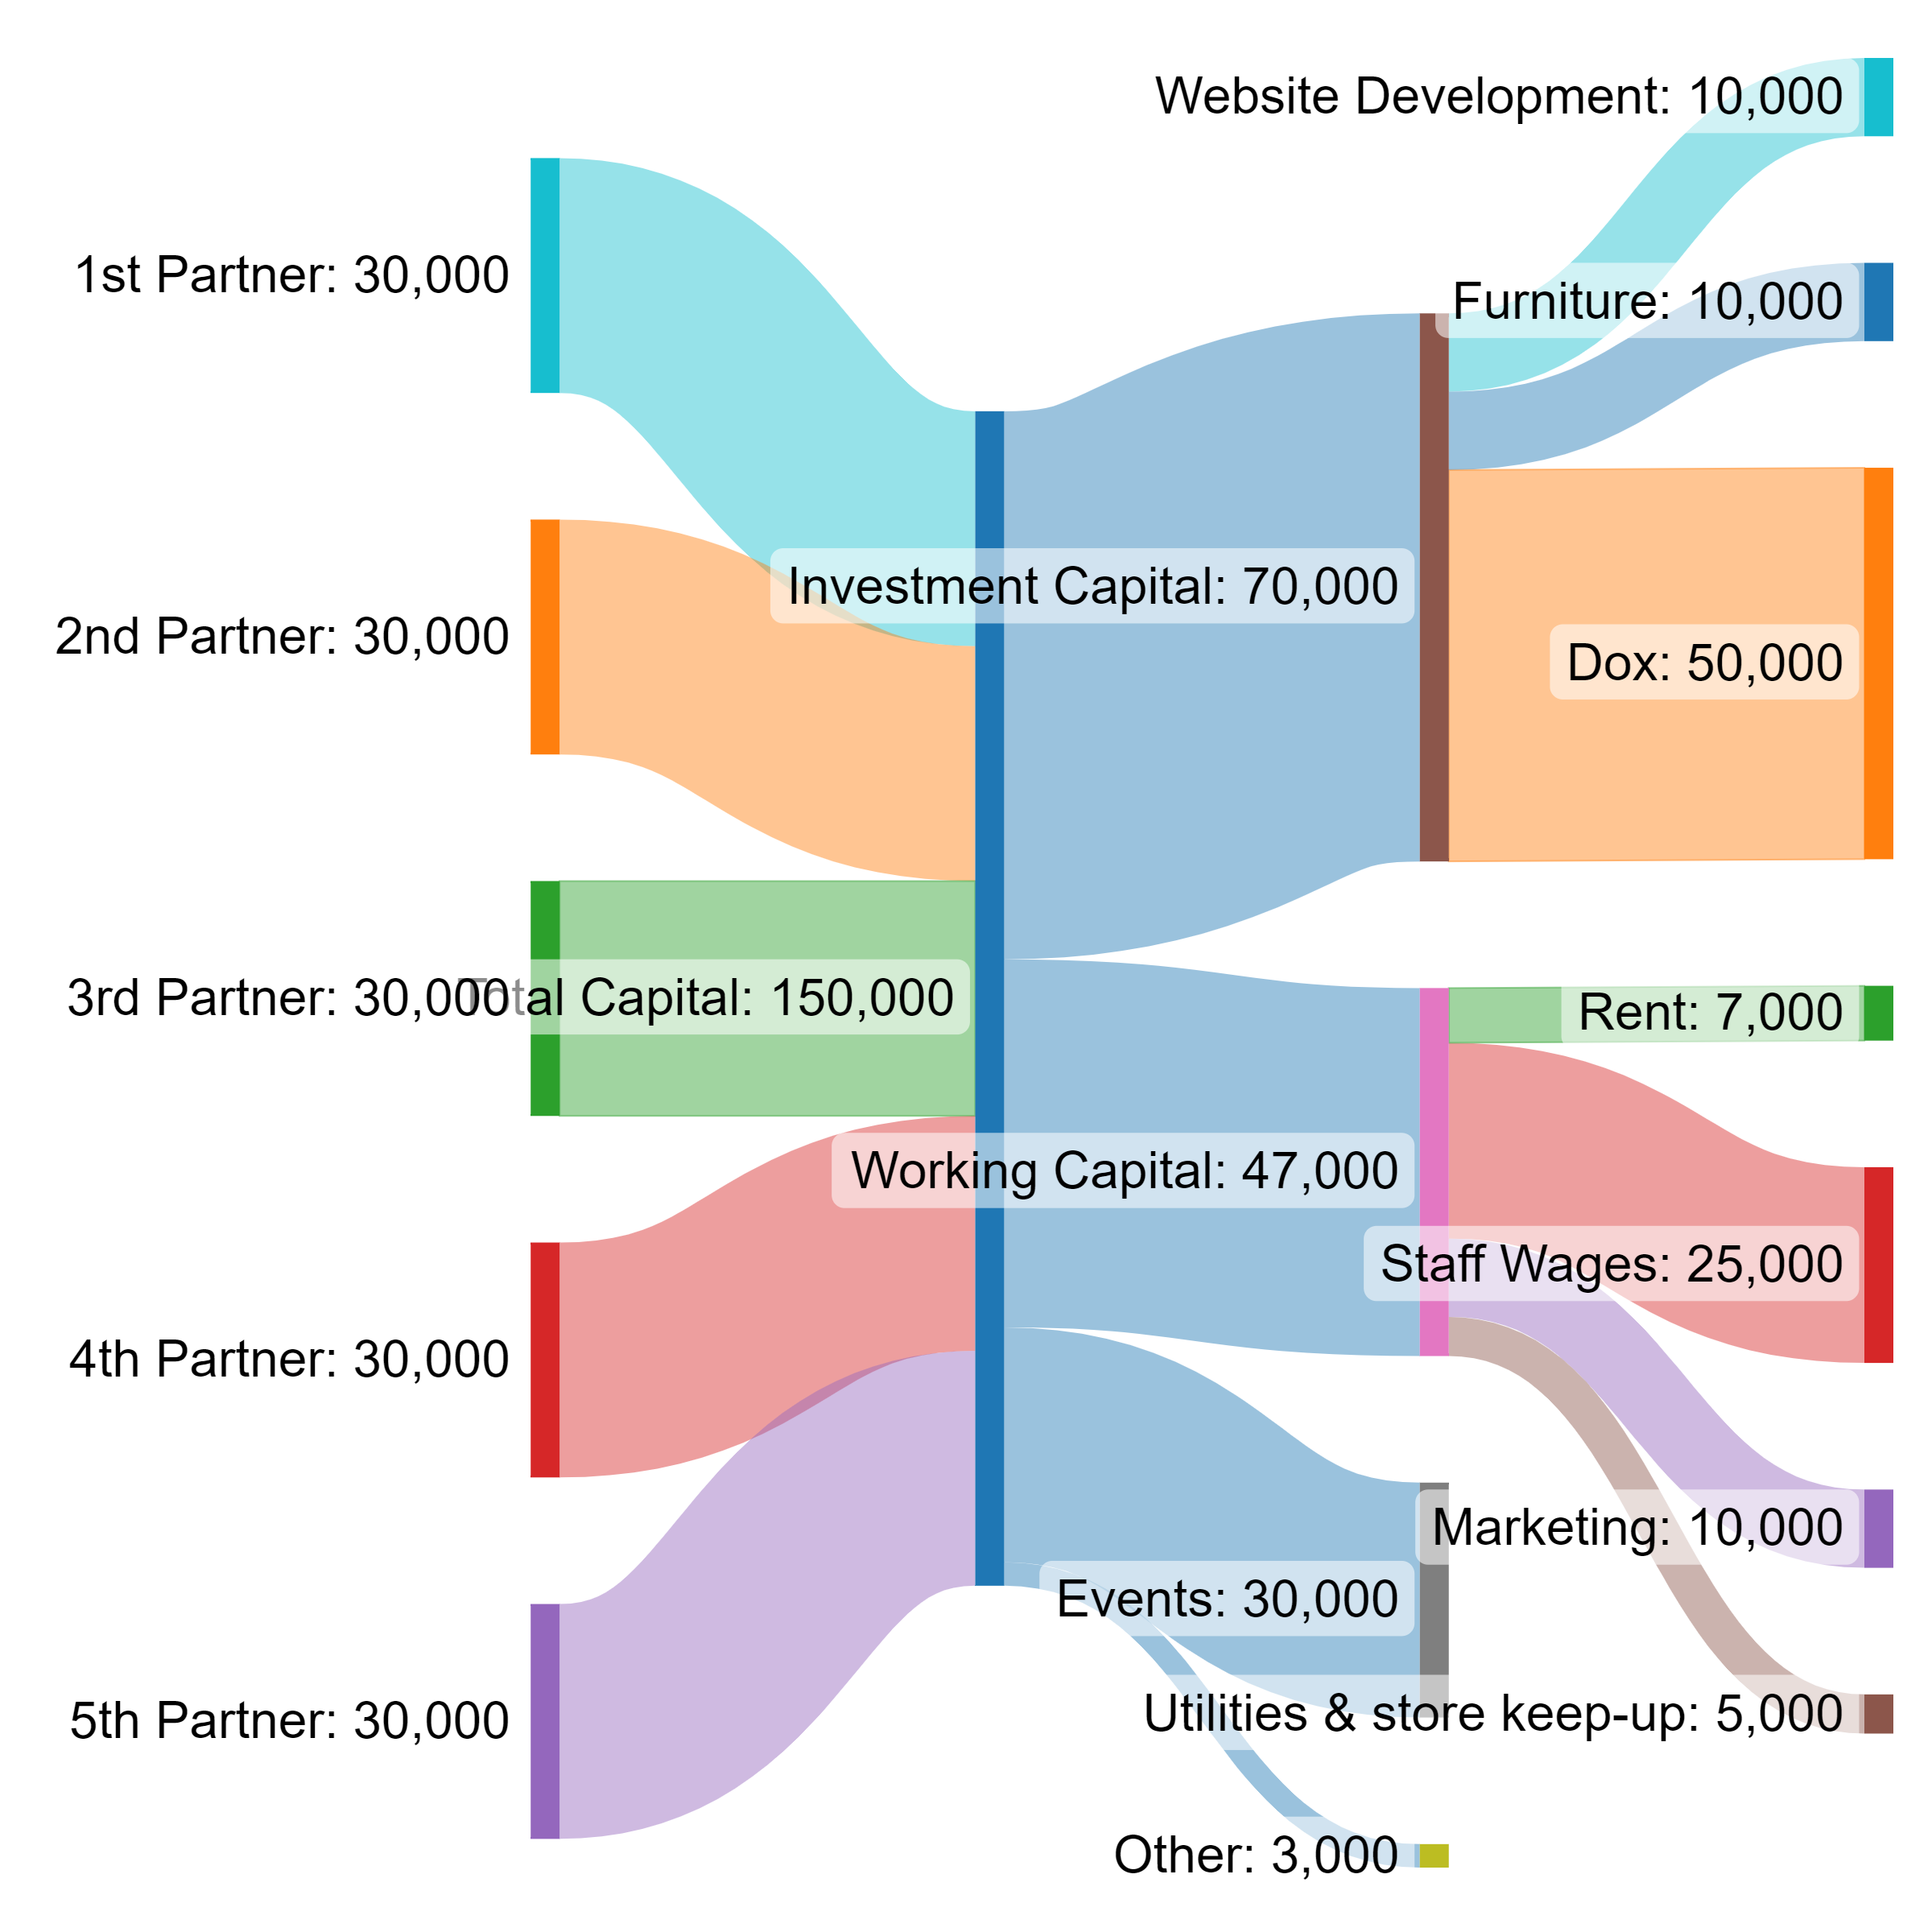
\includegraphics[scale=0.15]{capitalDistFlowDiagram.png}
    \caption{Flow Diagram of Touriscov's capital flow}
\end{figure}


\subsection{Revenue flow}
Touriscov's revenue is generated from many sources, but the prime of which comes from the cut it takes from its partners. And Touriscov's main business partners are airline companies, from which \tco\ makes its bulk revenue.\ \par

\noindent
The main monthly costs \tco\ deals with are the costs associated with its highly skilled staff. Those 25K are distributed as follows: 10K web developer, 6K customer service agent, 4K retail secretary, and 5K two documentation agents.\ \par
\vspace{2em}
\noindent
Below is a flow diagram of Touriscov's revenue streams and where that cash goes. The numbers are based on 3K website visitors per month with a 5\% conversion rate.\ \par

\noindent
\tco\ plans to reach that 3K website visitors number after about 2 month of its launch --- or even before that.\ \par


\begin{figure}[h]
    \centering
    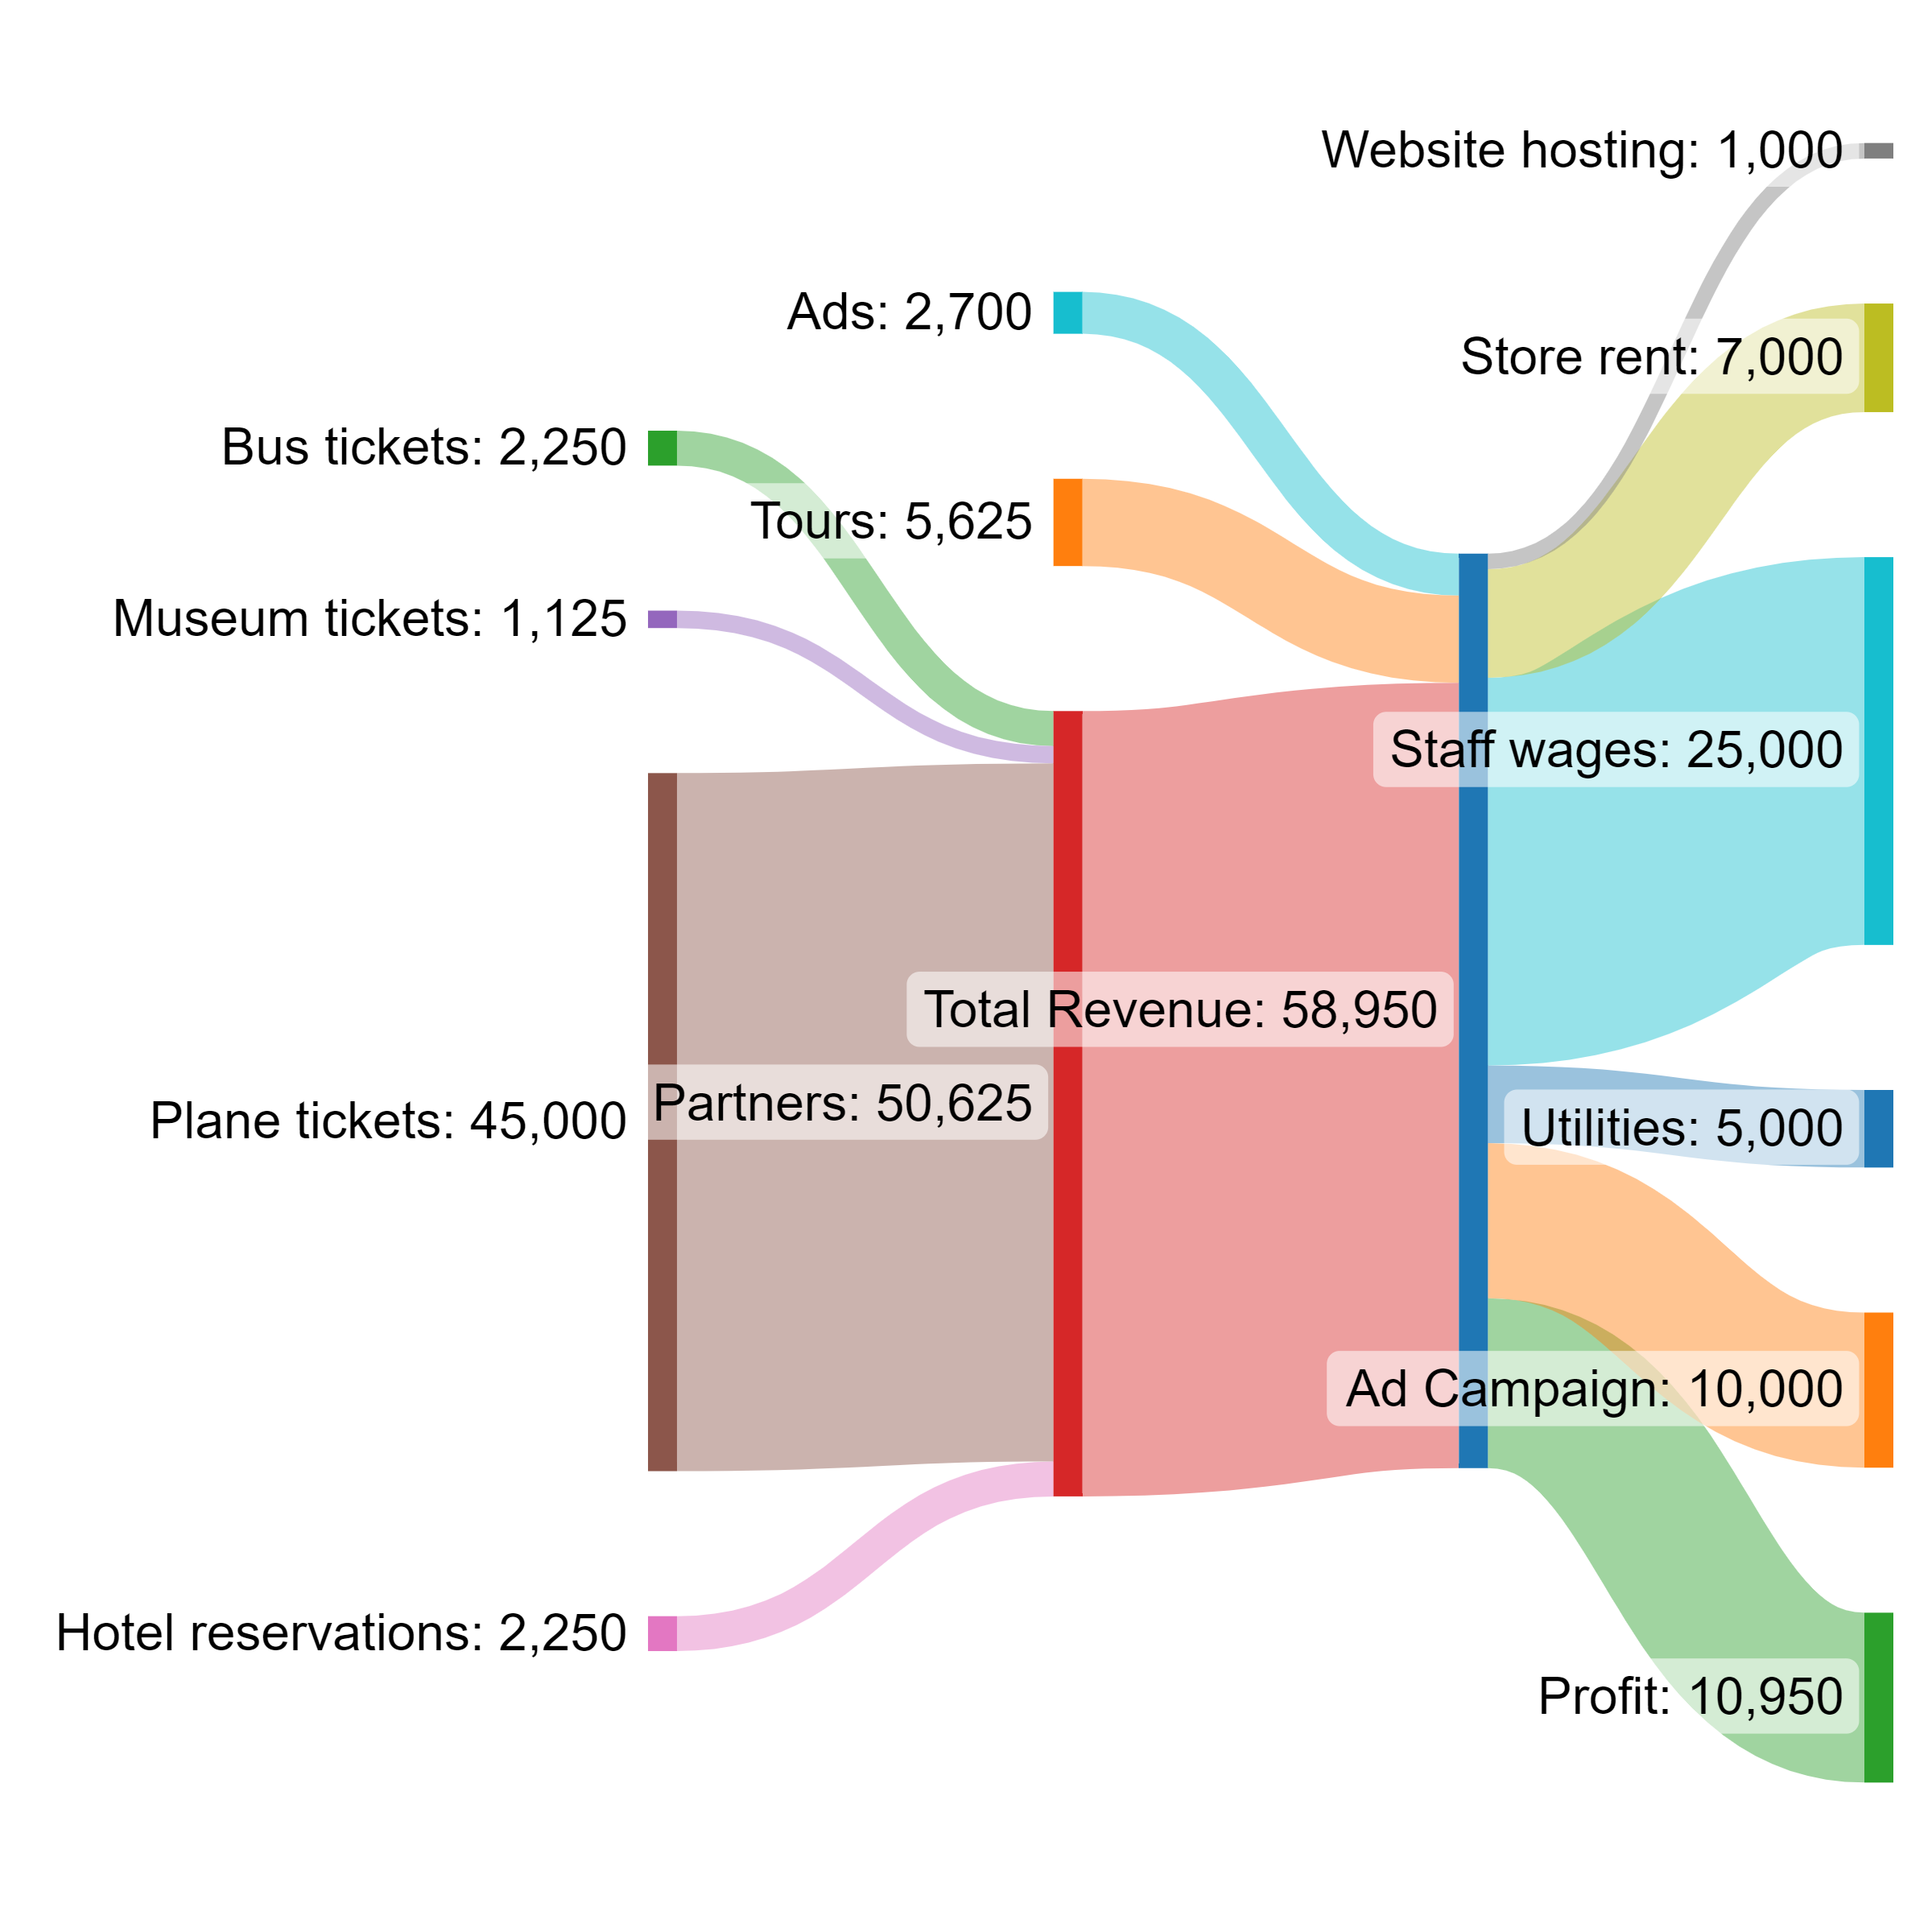
\includegraphics[scale=0.16]{newRevStreamsFlowDiagram.png}
    \caption{Flow Diagram of Touriscov's revenue sources}
\end{figure}

\subsection{Equilibrium Point}

\tco\ plans to make even (A.K.A reach its equilibrium point) after about 3 months of its launch. At that point, \tco\ expects to have about 4.5K monthly active users from which it plans to make about 59K total revenue.\ \par

\vspace{2em}

\begin{figure}[h]
    \centering
    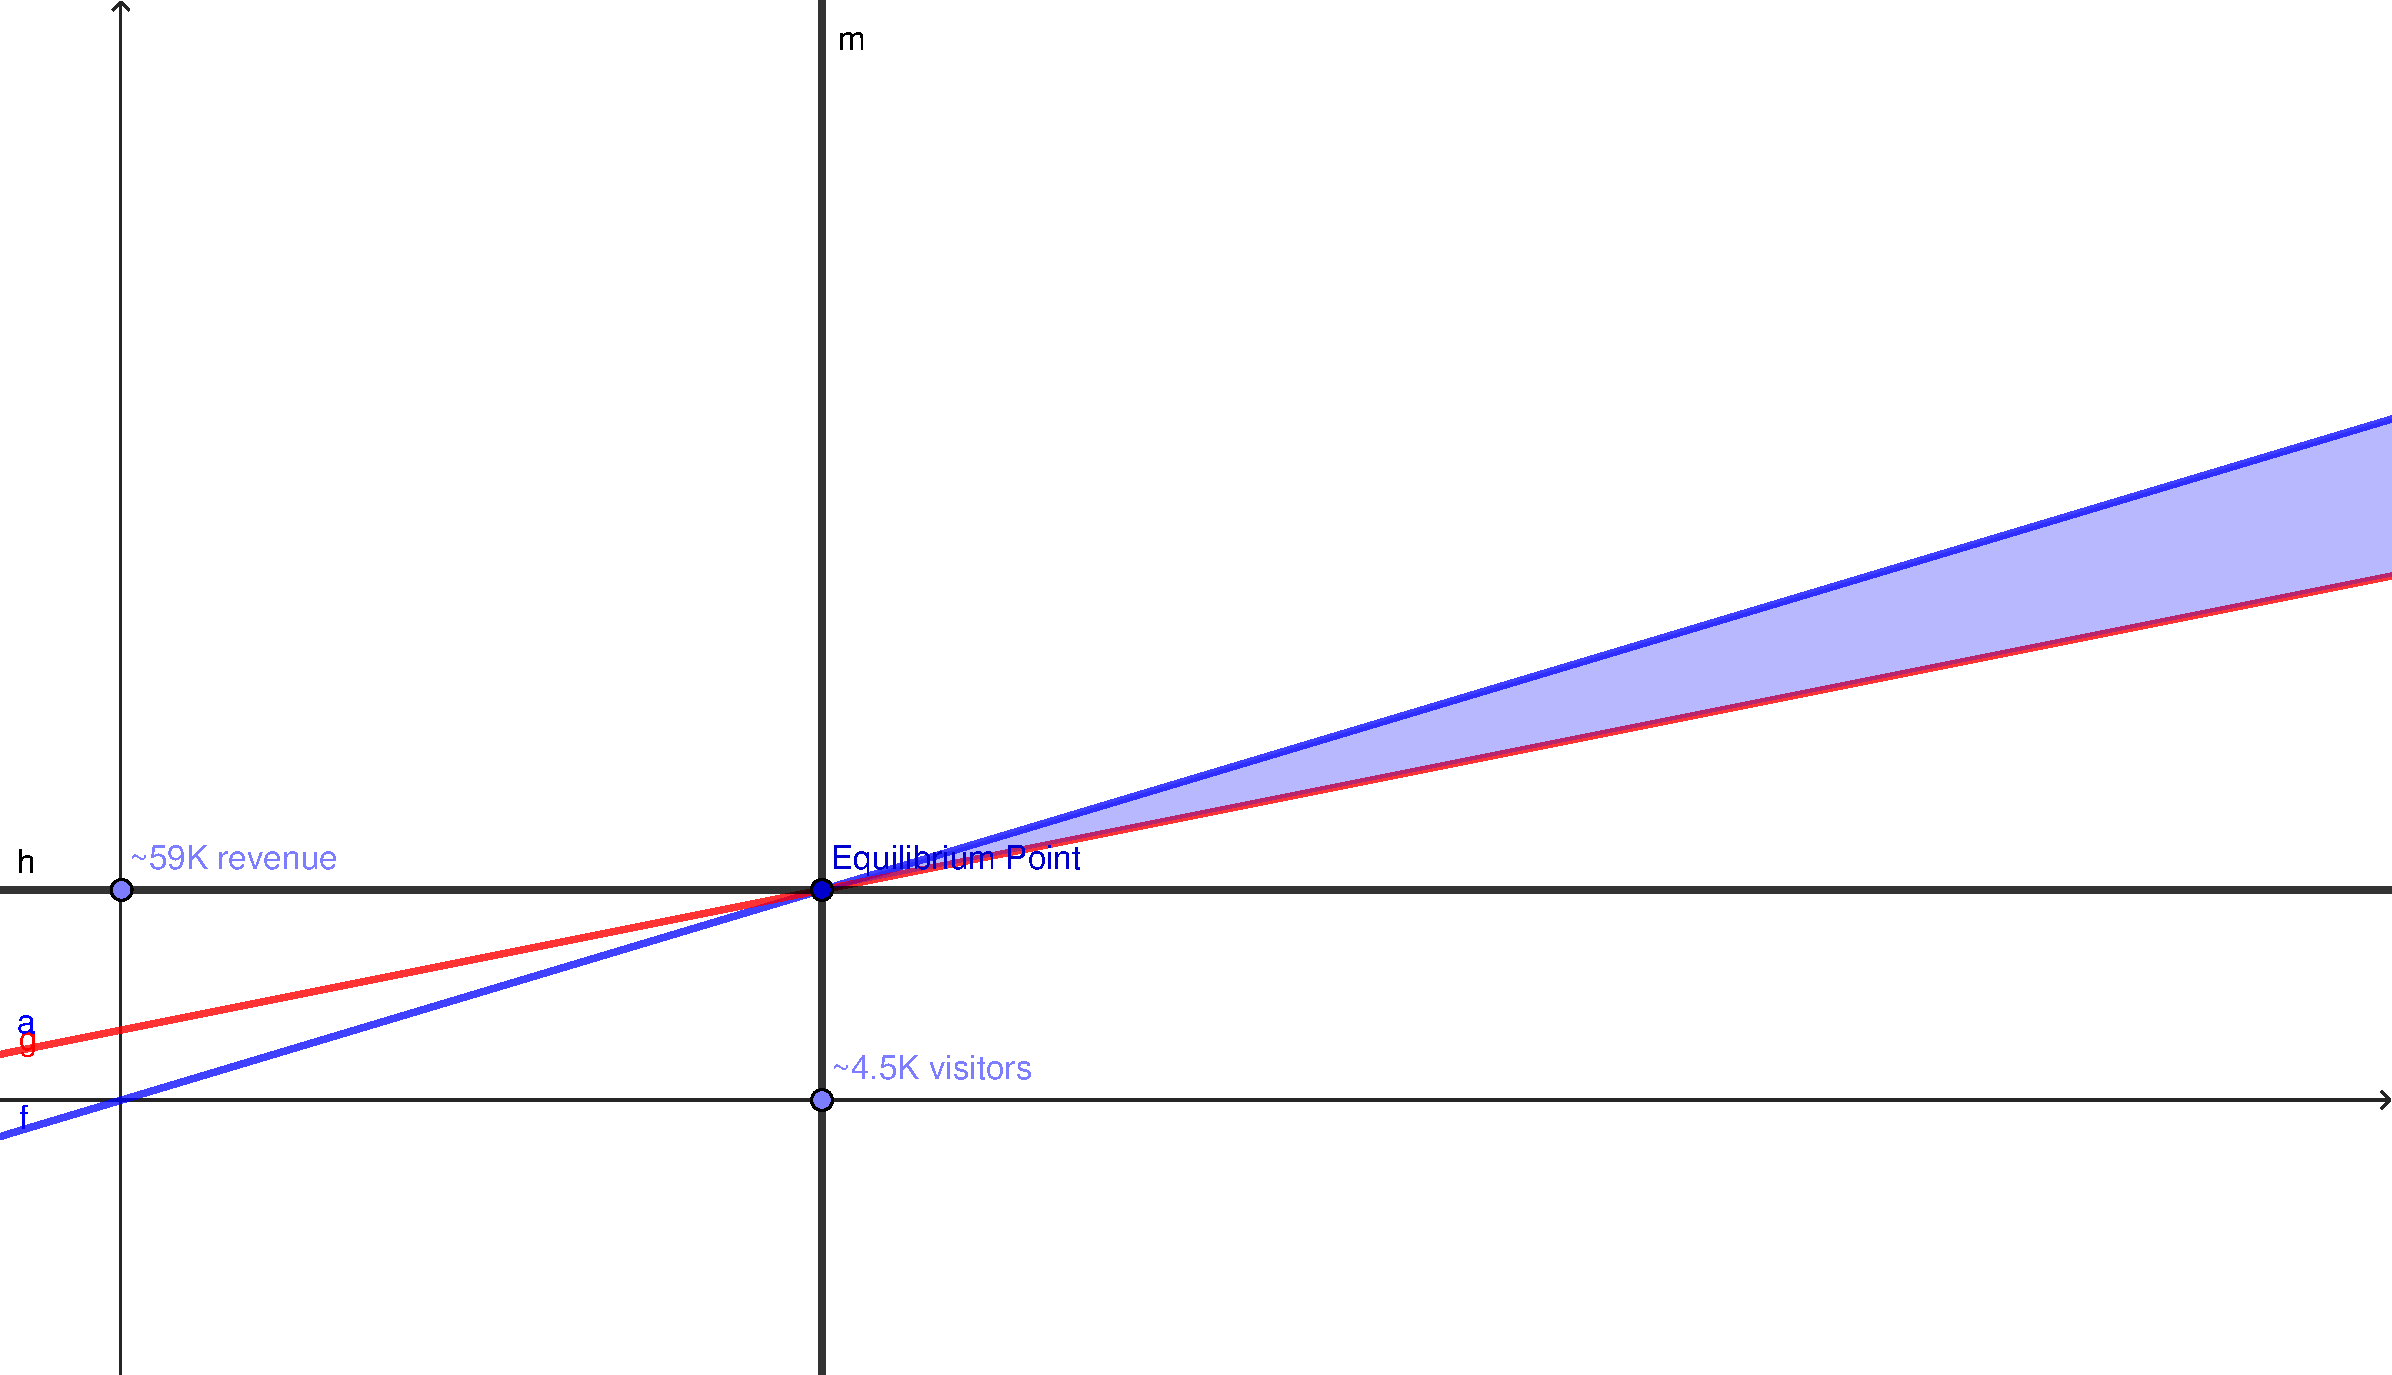
\includegraphics[scale=0.42]{equilibriumPoint.pdf}
    \caption{\tco\ equilibrium point diagram}
    \label{fig:my_label} % chktex 24
\end{figure}

\subsection{Taxes}
\tco\ is starting out as a partnership, so it is not subject to any corporate taxes. However, the owners of \tco\ are still subject to income taxes based on their country of residence respectively.\par

\noindent
Income tax for Egyptian residents is taken as a flat tax of 10\%

\hfill


\section{Appendix}
\begin{sidewaysfigure}
\begin{center}
        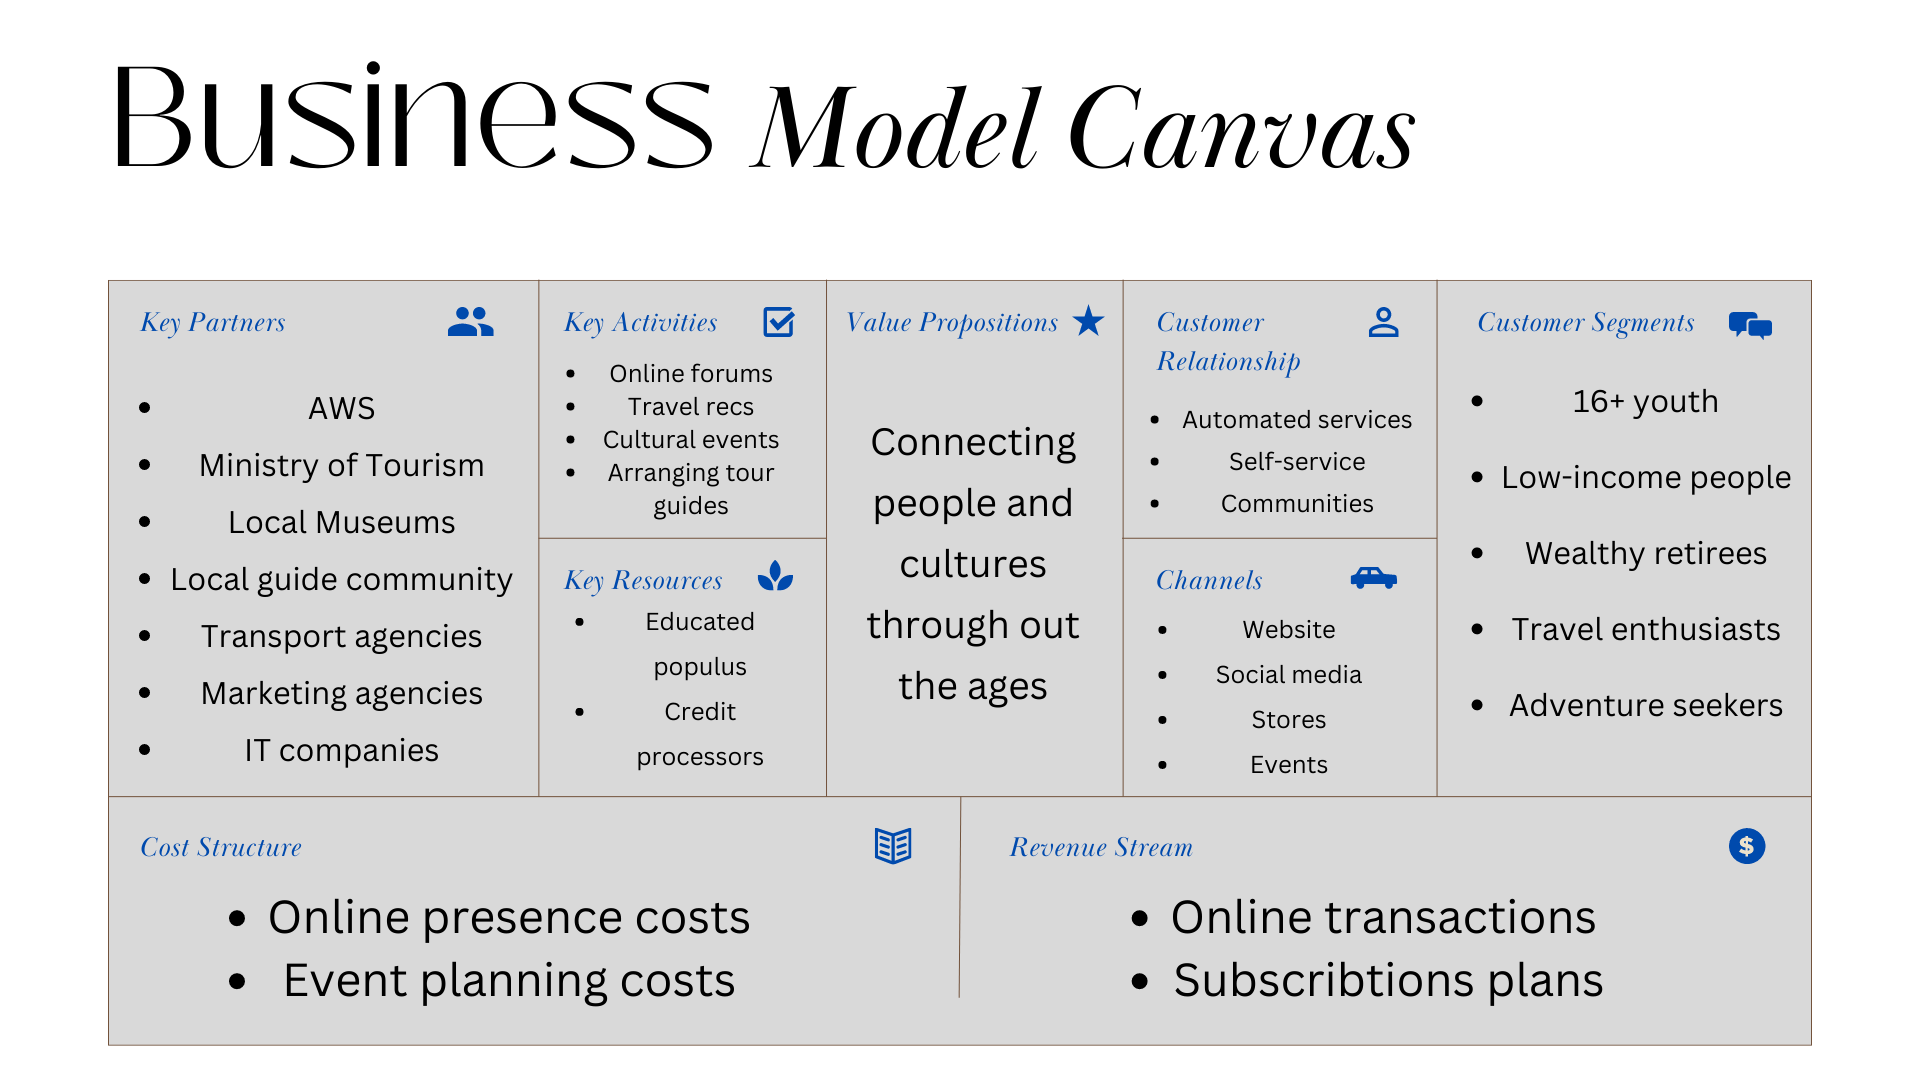
\includegraphics[width=0.92\textwidth]{businessModelCanvas.png}
\end{center}
\end{sidewaysfigure}

\begin{sidewaysfigure}
    \begin{center}
        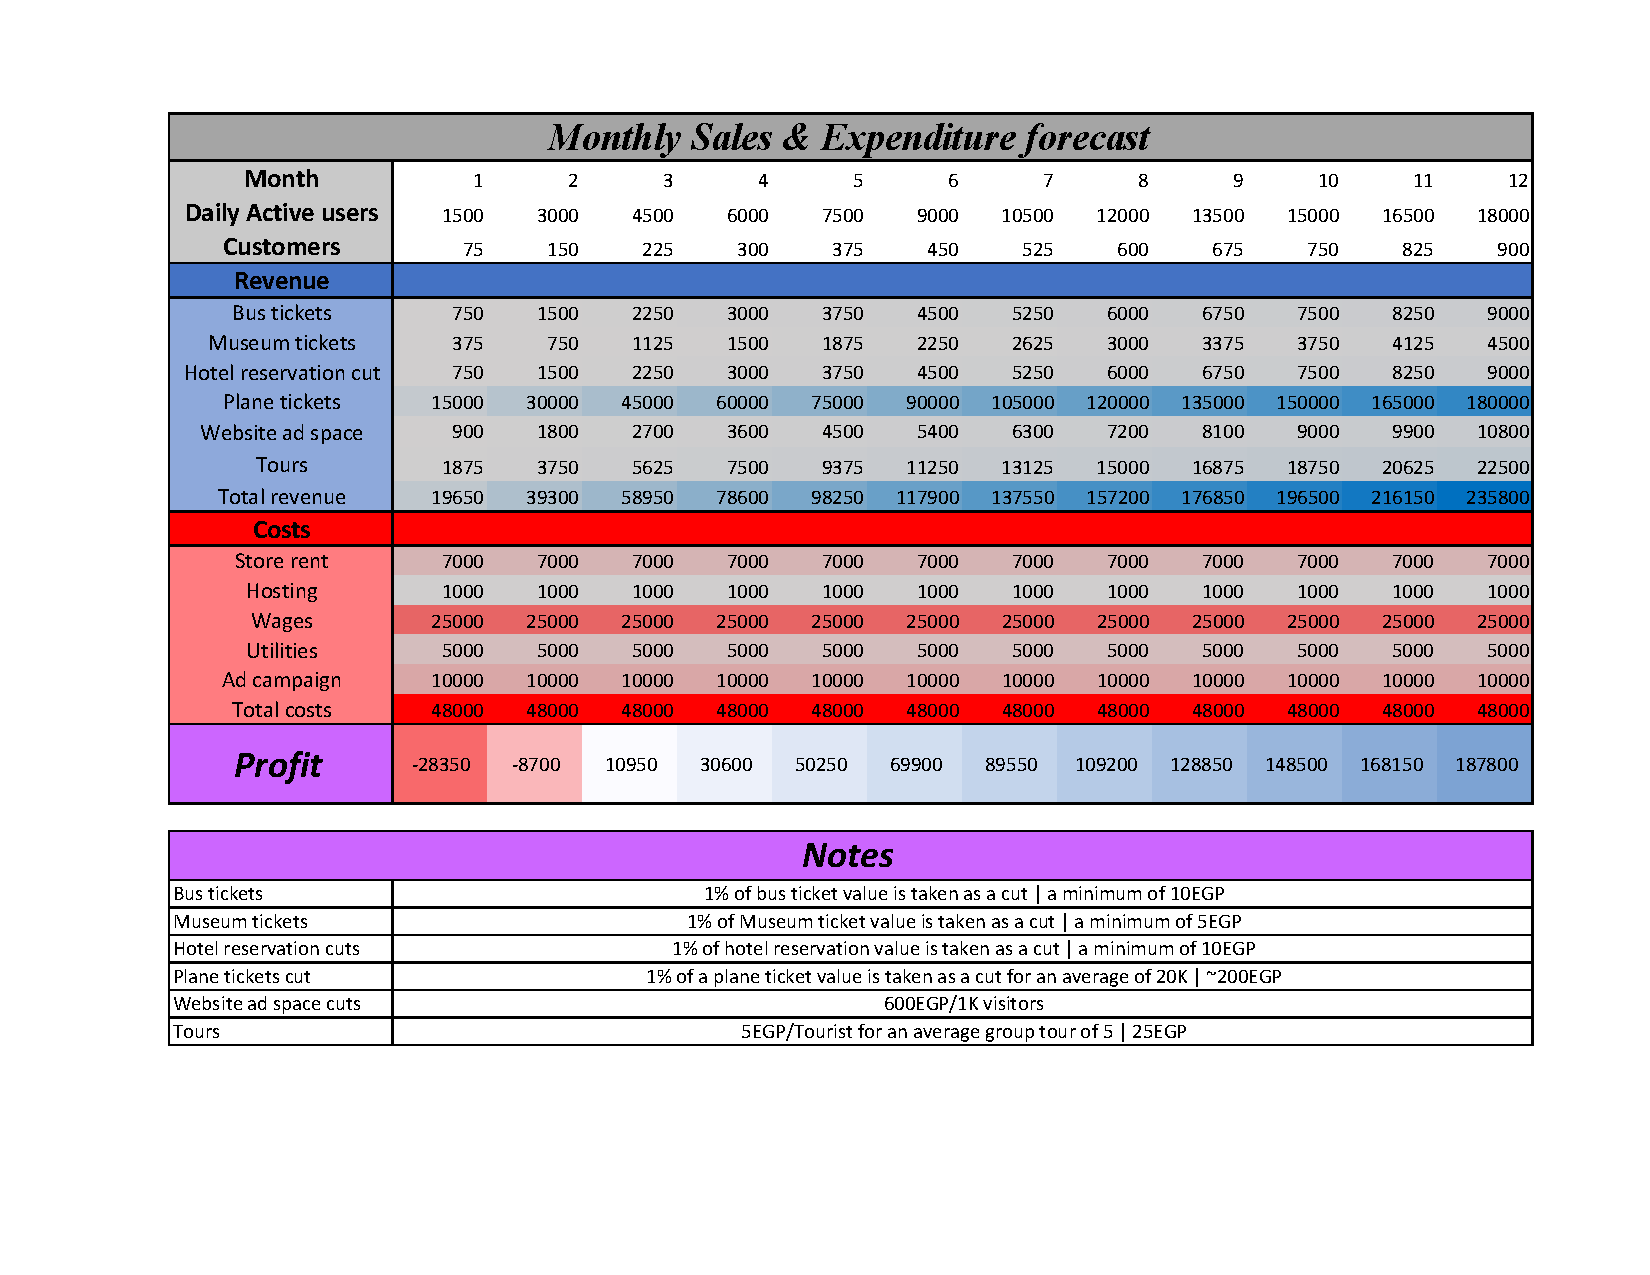
\includegraphics[width=\textwidth]{table1_miniMBA.pdf}
    \end{center}
\end{sidewaysfigure}

\begin{sidewaysfigure}
    \begin{center}
        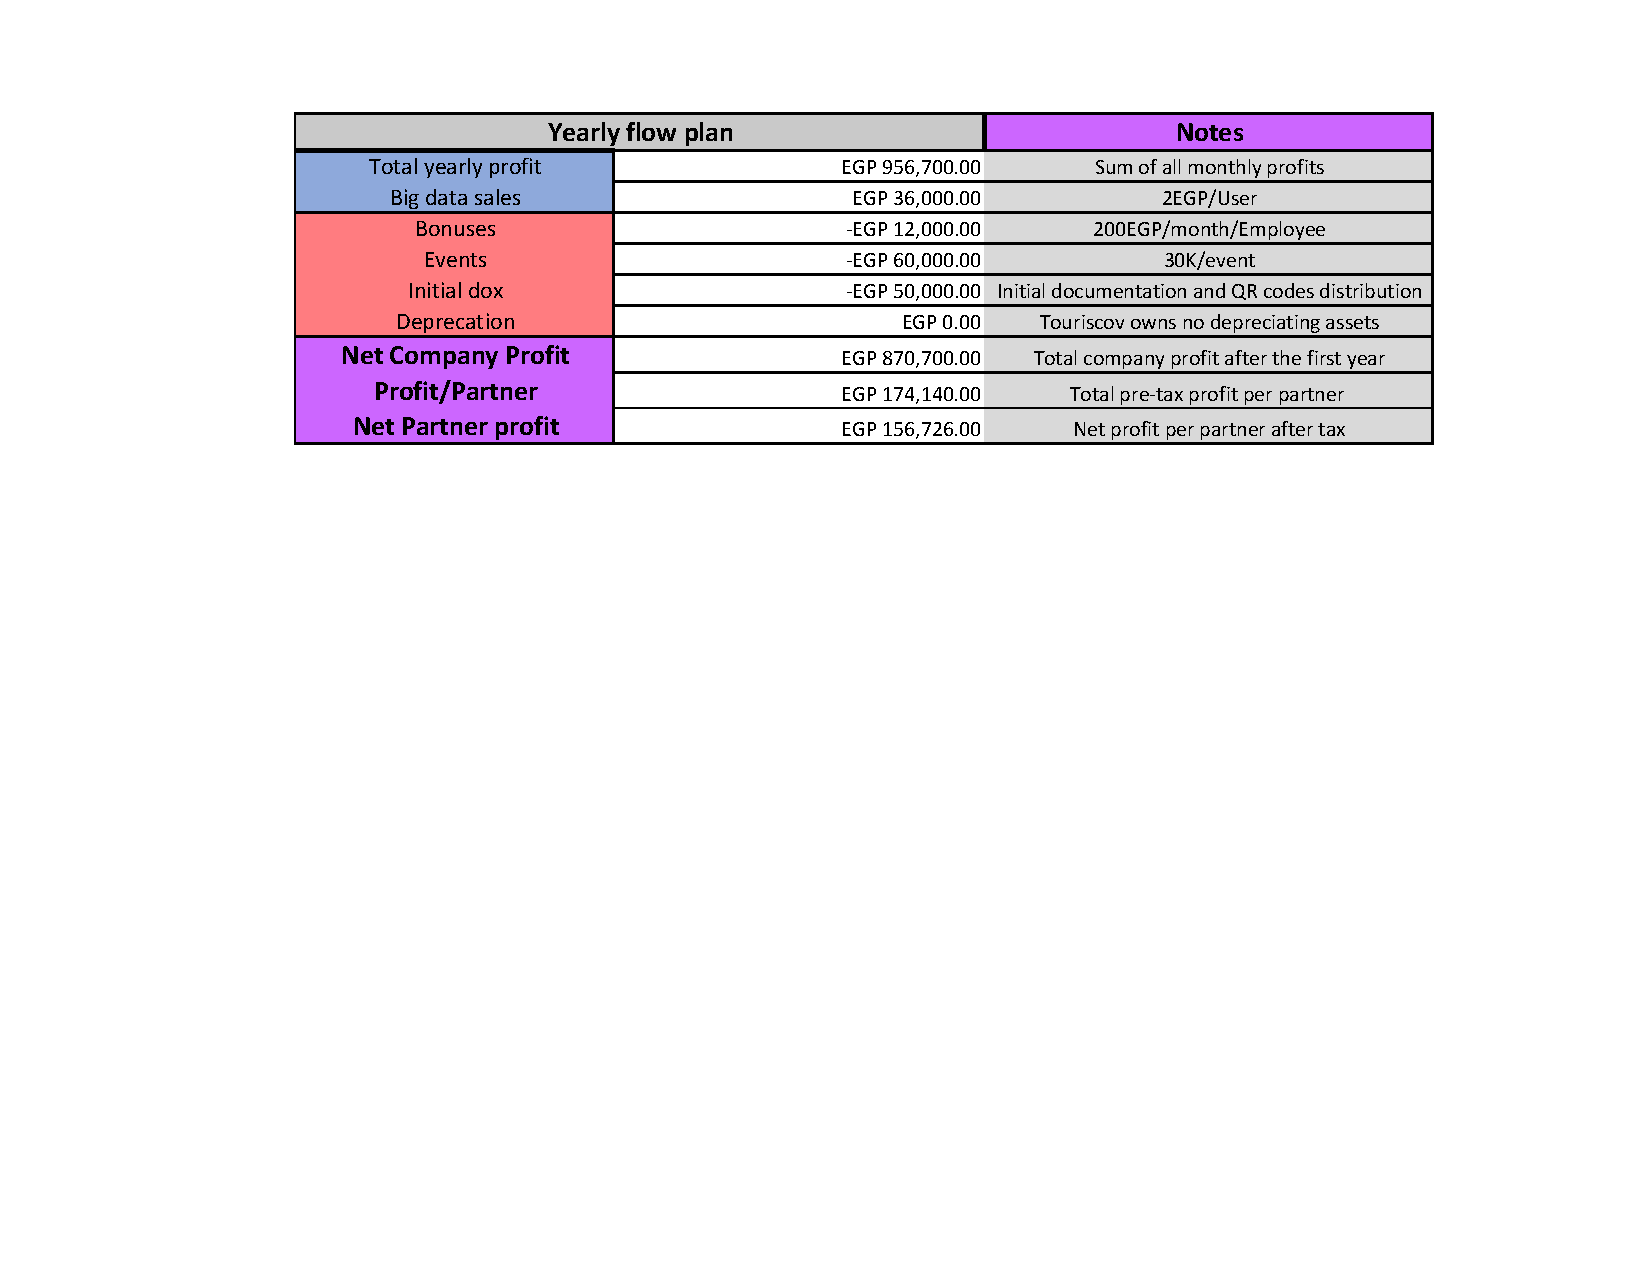
\includegraphics[width=\textwidth]{table2_miniMBA.pdf}
    \end{center}
\end{sidewaysfigure}
\end{document}
